\documentclass[12pt,a4paper]{report}

\usepackage{styles/dolgozat}

\usepackage{listings}
\usepackage{styles/cpp}
\usepackage{styles/python}

\usepackage{hyperref}
\usepackage{styles/dolgozat}
\begin{document}

\pagestyle{empty}

{\large
\begin{center}
\vglue 1truecm
\textbf{\huge\textsc{Szakdolgozat}}\\
\vglue 1truecm

\includegraphics[width=4.8truecm, height=4truecm]{images/me_logo.png}\\
\textbf{\textsc{Miskolci Egyetem}}
\end{center}}

\vglue 1.5truecm


{\LARGE
\begin{center}
\textbf{Ütközésvizsgálat automatikus optimalizálása térbeli modellekhez}
\end{center}}

\vspace*{2.5truecm}
{\large
\begin{center}
\begin{tabular}{c}
\textbf{Készítette:}\\
Szöllősi János\\
Programtervező informatikus
\end{tabular}
\end{center}
\begin{center}
\begin{tabular}{c}
\textbf{Témavezető:}\\
Dr. Nagy Noémi
\end{tabular}
\end{center}}
\vfill
{\large
\begin{center}
\textbf{\textsc{Miskolc, 2023}}
\end{center}}

\newpage


\newpage

\pagestyle{empty}

\begin{flushleft}
\textsc{\bfseries Miskolci Egyetem}\\
Gépészmérnöki és Informatikai Kar\\
Alkalmazott Matematikai Intézeti Tanszék\hspace*{4cm}\hfil \textbf{Szám:}
\end{flushleft}
\vskip 0.5cm
\begin{center}
\large\textsc{\bfseries Szakdolgozat Feladat}
\end{center}
\vskip 0.5cm
Szöllősi János (BC6X4X) programtervező informatikus jelölt részére.\newline

\noindent\textbf{A szakdolgozat tárgyköre:} Geometria, Optimalizálás\newline

\noindent\textbf{A szakdolgozat címe:} Ütközésvizsgálat automatikus optimalizálása térbeli modellekhez\newline

\noindent\textbf{A feladat részletezése:}

\medskip

\emph{A háromszögek metszésének számítása a számítógépi grafikában, térbeli modellezésben, szimulációkban egy gyakori probléma. A szakdolgozat az ehhez kapcsolódó számításokat, térpartícionálási és egyéb optimalizálási módszereket vizsgálja.}

\medskip

\emph{	A cél egy olyan függvénykönyvtár elkészítése, amely egy adott modell alapján létrehoz egy olyan struktúrát/objektumot, mely segítségével az ütközésdetektálás hatékonyan megoldható. A dolgozat bemutatja az elkészített algoritmusok működését, adatszerkezeteit, becslést ad a számítások idő- és tárigény komplexitására. A függvénykönyvtár C programozási nyelven készül, melyhez szemléltetés céljából OpenGL megjelenítés is tartozik.}

\vfill

\noindent\textbf{Témavezető:}Dr. Nagy Noémi (egyetemi adjunktus) \newline

\noindent\textbf{A feladat kiadásának ideje:} 2023. március 13.\newline

\vskip 2cm

\hbox to \hsize{\hfil{\hbox to 6cm {\dotfill}\hbox to 1cm{}}}

\hbox to \hsize{\hfil\hbox to 3cm {szakfelelős}\hbox to 2cm{}}

\newpage

\vspace*{1cm}  
\begin{center}
\large\textsc{\bfseries Eredetiségi Nyilatkozat}
\end{center}
\vspace*{2cm}  

Alulírott \textbf{Szöllősi János}; Neptun-kód: \texttt{BC6X4X} a Miskolci Egyetem Gépészmérnöki és Informatikai Karának végzős Programtervező informatikus szakos hallgatója ezennel büntetőjogi és fegyelmi felelősségem tudatában nyilatkozom és aláírásommal igazolom, hogy \textit{Ütközésvizsgálat automatikus optimalizálása térbeli modellekhez}
című szakdolgozatom saját, önálló munkám; az abban hivatkozott szakirodalom
felhasználása a forráskezelés szabályai szerint történt.\\

Tudomásul veszem, hogy szakdolgozat esetén plágiumnak számít:
\begin{itemize}
\item szószerinti idézet közlése idézőjel és hivatkozás megjelölése nélkül;
\item tartalmi idézet hivatkozás megjelölése nélkül;
\item más publikált gondolatainak saját gondolatként való feltüntetése.
\end{itemize}

Alulírott kijelentem, hogy a plágium fogalmát megismertem, és tudomásul veszem, hogy
plágium esetén szakdolgozatom visszautasításra kerül.

\vspace*{3cm}

\noindent Miskolc, \hbox to 2cm{\dotfill} .év \hbox to 2cm{\dotfill} .hó \hbox to 2cm{\dotfill} .nap

\vspace*{3cm}

\hspace*{8cm}\begin{tabular}{c}
\hbox to 6cm{\dotfill}\\
Hallgató
\end{tabular}



\newpage

\noindent 1.

\begin{tabular}{cl}
&szükséges (módosítás külön lapon) \\
A szakdolgozat feladat módosítása& \\
& nem szükséges\\
&\\
\hbox to 4cm{\dotfill}&\multicolumn{1}{c}{\hbox to 5cm{\dotfill}}\\
dátum& \multicolumn{1}{c}{témavezető(k)}
\end{tabular}
\vskip1.5mm

\noindent 2. A feladat kidolgozását ellenőriztem:

\vskip1.5mm

\begin{tabular}{l@{\hspace*{4cm}}l}
témavezető (dátum, aláírás):& konzulens (dátum, aláírás):\\
\dotfill&\dotfill\\
\dotfill&\dotfill\\
\dotfill&\dotfill
\end{tabular}

\vskip1.5mm

\noindent 3. A szakdolgozat beadható:

\vskip1.5mm

\begin{tabular}{@{\hspace*{1.3cm}}c@{\hspace*{2.1cm}}c}
\hbox to 4cm{\dotfill}&\multicolumn{1}{c}{\hbox to 5cm{\dotfill}}\\
dátum& \multicolumn{1}{c}{témavezető(k)}
\end{tabular}

\vskip1.5mm

\noindent 4.
\begin{tabular}[t]{@{}l@{\hspace*{1mm}}l@{\hspace*{1mm}}l@{}}
A szakdolgozat& \hbox to 3.5cm{\dotfill} &szövegoldalt\\
              & \hbox to 3.5cm{\dotfill} &program protokollt (listát, felhasználói leírást)\\
              &\hbox to 3.5cm{\dotfill}   &elektronikus adathordozót (részletezve)\\
              &\hbox to 3.5cm{\dotfill} & \\
              &\hbox to 3.5cm{\dotfill} &egyéb mellékletet (részletezve)\\
              &\hbox to 3.5cm{\dotfill} &\\
\end{tabular}
\newline tartalmaz.

\vskip1.5mm

\begin{tabular}{@{\hspace*{1.3cm}}c@{\hspace*{2.1cm}}c}
\hbox to 4cm{\dotfill}&\multicolumn{1}{c}{\hbox to 5cm{\dotfill}}\\
dátum& \multicolumn{1}{c}{témavezető(k)}
\end{tabular}

\noindent 5.

\begin{tabular}{ll}
&bocsátható\\
A szakdolgozat bírálatra& \\
& nem bocsátható\\
\end{tabular}

\vskip1.5mm

\noindent A bíráló neve: \hbox to 8cm{\dotfill}

\vskip4mm

\begin{tabular}{@{\hspace*{1.3cm}}c@{\hspace*{2.1cm}}c}
\hbox to 4cm{\dotfill}&\multicolumn{1}{c}{\hbox to 5cm{\dotfill}}\\
dátum& \multicolumn{1}{c}{szakfelelős}
\end{tabular}

\noindent 6.
\begin{tabular}[t]{@{}l@{\hspace*{1mm}}l@{\hspace*{1mm}}l@{}}
A szakdolgozat osztályzata& &\\
&a témavezető javaslata:& \hbox to 3cm{\dotfill}\\
&a bíráló javaslata:& \hbox to 3cm{\dotfill}\\
&a szakdolgozat végleges eredménye:& \hbox to 3cm{\dotfill}
\end{tabular}

\vspace*{4mm}

\noindent Miskolc, \hbox to 4.5cm{\dotfill} \hspace*{2.5cm}
\begin{tabular}[t]{cc}
\hbox to 6cm{\dotfill}\\
a Záróvizsga Bizottság Elnöke
\end{tabular}


\cleardoublepage
\pagenumbering{gobble}
\tableofcontents
\cleardoublepage
\pagenumbering{arabic}

\newpage

\pagestyle{fancy}

\Chapter{Bevezetés}

A szakdolgozat célja egy új függvénykönyvtár létrehozása, amely létrehoz automatikusan egy térbeli "hitboxot" a beimportált modellekhez, ezzel lehetővé téve a modellek közötti ütközések vizsgálatát. A szakdolgozathoz készített program \textbf{C} nyelven íródott \textbf{OpenGL} és \textbf{SDL2} függvénykönyvtárak segítségével. A program célja, hogy a modelleket felbontsa atomi szintre (háromszögekre), illetve a háromszögek metszéspontjainak kiszámításával pontos ütközésvizsgálat valósuljon meg.\\

Az ütközésvizsgálat, illetve "hitboxok" használata rendkívül fontos a számítógépes grafikában és a játékfejlesztésben. Játékok és fizikai szimulációk fejlesztése során rendkívül fontos, hogy a modellek ütközésvizsgálata megbízható és pontos legyen. A szakdolgozatban szereplő algoritmus a pontosságot célozza meg.\\

Az atomi szintű ütközésvizsgálat során nagy pontosságot érhetünk el, ezzel valósághű és precíz számításokat, szimulációkat végezhetünk el. A szakdolgozat során részletesen bemutatásra kerül a függvénykönyvtár tervezése, illetve implementációja.\\

A fejezetek végigvezetnek a függvénykönyvtár alapvető működésétől, a részletes implementáción át az optimalizációs lehetőségekig, valamint a függvénykönyvtár használatára is kitérnek. A szakdolgozat eredménye egy olyan függvénykönyvtár, amely hozzájárul a játékfejlesztés, illetve számítógépes grafika lehetőségeinek kibővítéséhez, ezzel segítve a fejlesztőket a kidolgozott hatékony ütközésvizsgálati megoldással.
\Chapter{Koncepció}

A feladat fő problémája a háromszögek metszéspontjának kiszámítása a térben. Ez sajnos nem egy egyszerű feladat. Programozás terén, illetve erőforrásigény terén sem elhanyagolható.

A valóságban az emberi gondolkodásnak egyszerűnek tűnhet eldönteni, hogy két háromszög metszi-e egymást, vagy sem. Programozás, illetve matematika terén viszont sokkal nehezebb. Rengeteg számítást kell végeznünk ahhoz, hogy megbizonyosodjunk a háromszögek metszéséről.

\Section{Irodalomkutatás}
A metszéspontok számításhoz legmegfelelőbbnek \textbf{\href{https://www.geometrictools.com/Documentation/DynamicCollisionDetection.pdf}{David Eberly 1999-es kutatását}}, azon belül a \cite{triangles}(4.1 Separation of Triangles) szekciót találtam. A dokumentáció tökéletesen elmagyarázza a matematikai képletek elemeit, azok használatát, lépéseit. Ezek mind táblázatba szedve találhatóak. A pontos magyarázat a következő fejezetben található. Emellett rengeteg különböző módszer található az interneten térbeli modellek ütközésének vizsgálatához, például:\\
\newpage
\subsection{Négyzetes elválasztás:}
A négyzetes elválasztás módszere egy olyan algoritmus, amelyet számítógépes játékok, illetve számítógépi grafikában közkedvelten használnak ütközések érzékelésére.
A módszer segítségével meghatározhatjuk, hogy két vagy több modell metszik-e egymást vagy sem.
Az ötlet lényege, hogy minden modellt négyzet alakú "dobozokkal" vesszük körbe, amelyet a legkisebb négyszögű terület alapján határozzuk meg. Ekkor az ütközést csak akkor kell ellenőrizni, ha a meghatározott "dobozok" metszik egymást.\\
Lépései:

\textbullet Minden modellhez rendelünk egy "dobozt", amely a legkisebb területen határozza meg a modellt. Ez a "doboz" könnyen meghatározható 4 ponttal a térben.\\

\textbullet Ellenőrizzük a "dobozokat", hogy metszik-e egymást vagy sem.\\

\textbullet Ha két vagy több "doboz" metszik egymást, akkor kerül sor a pontos ütközésvizsgálatra (jelen szakdolgozat alapján ez háromszögek metszéspontjának számítása).\\

Előnye a módszernek, hogy a bonyolult modelleket leírhatjuk először egyszerű geomatria alakzattal, így az ütközésvizsgálat ideje nagyban csökken.

Hátránya a módszernek, hogy az algoritmus csak közelíti az eredményt, ezért fontos egyéb algoritmusokat alkalmazni a pontos ütközésvizsgálathoz.

\subsection{Sugárkövetés módszere:}
A sugárkövetés módszere egy nagyon elterjedt technológia ütközések vizsgálatához. Ezzel a módszerrel valós időben tudjuk kiszámítani a világítást és az árnyékokat.
Az ötlet lényege, hogy a modellek és a fényforrások közötti interakciókat számítjuk. Egy sugarat bocsátunk ki a képpont irányába a kamera pozíciójából, és ellenőrizzük, hogy a sugár milyen modelleket metsz.
Így meg tudjuk határozni, hogy a képpont milyen modelltől kap fényt, illetve milyen árnyékokat, színeket szükséges megjeleníteni.
\\
Lépései:

\textbullet Létrehozzuk a sugarat minden képpontra a kamera pozíciójából. Így a sugár meghatározza a képpont irányát, illetve pozícióját.\\

\textbullet Végighaladunk a sugár útján és ellenőrizzük milyen modellek metszik a sugarat.\\

\textbullet Amikor a sugár metsz egy modellt, akkor kiszámítjuk az anyagtulajdonságokat. Például fényvisszaverődés, színek, tükröződés, árnyékolás.\\

\textbullet A modellek és a fényforrások közti távolságok, illetve átlátszóságok alapján kiszámítjuk, hogy az adott pontba mennyi fény jut.\\

\textbullet Néhány esetben továbbfejleszthető a módszer rekurzióval. Ez azt jelenti, hogy ha a sugár ütközik egy modellel, akkor további sugarakat hozunk létre. Ezzel részletesebb tükröződéseket hozhatunk létre.\\

Előnye a módszernek, hogy hatékonyan hozhatunk létre fotorealisztikus képeket.

Hátránya a módszernek, hogy a számítási igénye magas.


\subsection{Voxel-alapú:}
A voxel-alapú módszer egy hatékony módszer, amely a háromdimenziós teret felosztja kisebb részekre. A teret téglalap alakú részekre bontja, ezeket a részeket voxel-nek nevezzük.
Ezekkel a voxelekkel közelítjük a modelleket.
\\
Lépései:

\textbullet Voxel rácsot hozunk létre. Ezzel a ráccsal osztjuk fel a teret kisebb voxelekre. Ez egy háromdimenziós rács szerkezet.\\

\textbullet A modelleket voxelekkel közelítjük, amelyek a voxel rácsban helyezkednek el. A pontosság módosítható a voxelek mérete alapján. Minden voxelt megjelöljük az alapján, hogy tartalmaz-e modellt vagy sem.\\

\textbullet Ütközések vizsgálatához azt ellenőrizzük, hogy a két modellt tartalmazó voxel metszik-e egymást vagy sem. Ha egy aktív voxel metszi a másik aktív voxelt, akkor a modellek ütközhetnek egymással. Ezután szükséges egyéb ütközésvizsgálat a pontosításhoz.\\

Előnye a módszernek, hogy a használata egyszerű, a pontosság könnyen módosítható. Nagyobb tér esetén hatékony megoldás lehet. Az ütközésvizsgálat csak az aktív voxelek esetén történik meg, így elkerülhető a fölösleges számítások.

Hátránya a módszernek, hogy nehéz pontosan meghatározni a voxel rács méretét. Túl nagy méret esetén az ütközésvizsgálat nem lesz elég pontos, kis méret esetén a számítások költségesek lehetnek.

\subsection{Egyenletek alkalmazása:}
Az egyenletek alkalmazásának módszere egy elterjedt technológia. A módszer alapötlete, hogy matematikai egyenletek segítségével határozza meg a modellek mozgásának, illetve ütközéseinek érzékelésére.
\\
Lépései:

\textbullet Felállítunk egy matematikai modellt, amely leírja a modellek mozgását.\\

\textbullet Definiáljuk az ütközések vizsgálatához szükséges szabályokat, feltételeket. Ezek a feltételek lehetnek egyszerűbbek, vagy komplexebbek, például távolságok, sebességek, fizikai tulajdonságok, formák, méretek.\\

\textbullet A meghatározott modell és a feltételek alapján ellenőrizzük az ütközésvizsgálatot.\\

\textbullet Gyakran szükség van az egyenletek alkalmazására numerikus módszerekre, például differenciálegyenletek megoldása esetén.\\

Előnye a módszernek, hogy pontos fizikai szimulációkat érzékelhetünk.

Hátránya a módszernek, hogy magas a számítási igénye, ezért nem alkalmas valós idejű szimulációkra, illetve magas modellszám esetén sem előnyös.
\Chapter{Ütközések számítása}
\label{chap:utkozesek}
A háromszöget metszéspontjának számításához elsősorban szükségünk van 2 háromszögre, mint input. Ezek csúcspontjait jelöljük az $\textbf{A}_0$, $\textbf{A}_1$, $\textbf{A}_2$, illetve $\textbf{B}_0$, $\textbf{B}_1$, $\textbf{B}_2$ pontokkal. A csúcspontok segítségével kiszámíthatjuk a háromszögek éleit. Ezek lesznek a $\textbf{C}_0$, $\textbf{C}_1$, $\textbf{C}_2$, illetve $\textbf{E}_0$, $\textbf{E}_1$, $\textbf{E}_2$ élek: \\
$$\textbf{C}_0 = \textbf{A}_1 - \textbf{A}_0, \textbf{C}_1 = \textbf{A}_2 - \textbf{A}_0, \textbf{C}_2 = \textbf{C}_1 - \textbf{C}_0 .$$\\
Az élek segítségével kiszámíthatjuk a háromszögek normál vektorait. Ezek lesznek a \textbf{D}, illetve \textbf{F} vektorok:  \\
$$\textbf{D = C}_0 \times \textbf{C}_1,\textbf{F = E}_0 \times \textbf{E}_1.$$\\
A számítások megkönnyítéséhez kiszámítjuk az eltolásvektort is:  \\
$$\textbf{G = B}_0 -\textbf{A}_0.$$\\
Ezen adatok szolgálják az alapokat, amelyekből további számításokat végzünk. A metszés eldöntéséhez a következő univerzális képletet használjuk:\\
\hbox to 6cm{}	$\textbf{H}_1 = \textbf{L * C}_0,$\\
\hbox to 6cm{}	$\textbf{H}_2 = \textbf{L * C}_1,$\\
\hbox to 6cm{}	$\textbf{I}_0 = \textbf{L * G},$\\
\hbox to 6cm{}	$\textbf{I}_1 = \textbf{I}_0 + \textbf{L * E}_0,$\\
\hbox to 6cm{}	$\textbf{I}_2 =\textbf{ I}_0 + \textbf{L * E}_1.$\\

Minden sor 1-1 számítást jelent. Minden számítás után ellenőriznünk kell, hogy a két adott háromszög metszi-e egymást, vagy sem. Erre a következő képletet használjuk: Ha\\
$$\textbf{min(H) > max(I) vagy max(H) < min(I)},$$akkor a két háromszögre biztosan mondható, hogy nem metszik egymást. Ez esetben nem szükséges további számításokat végezni. Amennyiben nemleges választ kapunk, akkor tovább kell számítanunk minden sort. Ha az utolsó sor esetén sem kapunk pozitív választ, akkor kimondhatjuk, hogy a két háromszög metszi egymást. A pontos matematikai számításokat a \ref{tab:szamitas} táblázat mutatja.

\newpage

\begin{table}
	\centering
	
	\begin{tabular}{|c||c|c|c|c|c|}
		\hline
		\textbf{L}     & $\textbf{H}_1$   & $\textbf{H}_2$    & $\textbf{I}_0$      & $\textbf{I}_1$        & $\textbf{I}_2$        \\ \hline
		\textbf{D}     & 0    & 0     & D*G     & I0 + D*$E_0$ & I0 + D*$E_1$ \\ \hline
		\textbf{F}     & F*$C_0$ & F*$C_1$  & F*G     & $I_0$        & $I_0$        \\ \hline
		$\textbf{C}_0$*$\textbf{E}_0$ & 0    & -D*$E_0$ & $C_0$$\times$$E_0$*G & $I_0$        & $I_0$ + F*$C_0$ \\ \hline
		$\textbf{C}_0$*$\textbf{E}_1$ & 0    & -D*$E_1$ & $C_0$$\times$$E_1$*G & $I_0$ - F*$C_0$ & $I_0$        \\ \hline
		$\textbf{C}_0$*$\textbf{E}_2$ & 0    & -D*$E_2$ & $C_0$$\times$$E_2$*G & $I_0$ - F*$C_0$ & $I_1$        \\ \hline
		$\textbf{C}_1$*$\textbf{E}_0$ & D*$E_0$ & 0     & $C_1$$\times$$E_0$*G & $I_0$        & $I_0$ + F*$C_1$ \\ \hline
		$\textbf{C}_1$*$\textbf{E}_1$ & D*$E_1$ & 0     & $C_1$$\times$$E_1$*G & $I_0$ - F*$C_1$ & $I_0$        \\ \hline
		$\textbf{C}_1$*$\textbf{E}_2$ & D*$E_2$ & 0     & $C_1$$\times$$E_2$*G & $I_0$ - F*$C_1$ & $I_1$        \\ \hline
		$\textbf{C}_2$*$\textbf{E}_0$ & D*$E_0$ & $H_1$    & $C_2$$\times$$E_0$*G & $I_0$        & $I_0$ + F*$C_2$ \\ \hline
		$\textbf{C}_2$*$\textbf{E}_1$ & D*$E_1$ & $H_1$    & $C_2$$\times$$E_1$*G & $I_0$ - F*$C_2$ & $I_0$        \\ \hline
		$\textbf{C}_2$*$\textbf{E}_2$ & D*$E_2$ & $H_1$   & $C_2$$\times$$E_2$*G & $I_0$ - F*$C_2$ & $I_1$        \\ \hline
	\end{tabular}
	\caption{A számítások táblázata.}
	\label{tab:szamitas}
\end{table}

\newpage

\Section{Függvénykönyvtár tervezése}
A függvénykönyvtár C nyelven \cite{C} íródott C11 szabványban. Ez egy egyszerűen megtanulható, gyors programozási nyelv. Létrehozhatunk benne függvényeket, új típusokat/struktúrákat, amelyet később bárhol használhatunk a program készítése során. A készített függvénykönyvtár könnyen használható, mindössze bele kell raknunk az általunk készített program forráskódjai közé a collision\_triangle.c, illetve collision\_triangle.h fájlokat, majd beimportálni azt a forráskódban a '\#include "collision\_triangle.h"' sor segítségével. Ha mindent helyesen csináltunk, akkor máris használhatóak a függvények, illetve struktúrák, amelyeket a \ref{tab:strukt}, illetve \ref{tab:fug} táblázat mutatja be.


\begin{table}[h]
	\centering
	\begin{tabular}{|c|c|c|}
		\hline
		\textbf{Változó}     & \textbf{Típusa}& \textbf{Leírása}\\ \hline
		x&Float&Egy háromdimenziós pont helyét jelöli az x tengelyen.\\ \hline
		y&Float&Egy háromdimenziós pont helyét jelöli az y tengelyen.\\ \hline
		z&Float&Egy háromdimenziós pont helyét jelöli az z tengelyen.\\ \hline
		
	\end{tabular}
	\caption{Vec3 struktúra bemutatása}
	\label{tab:strukt}
\end{table}

\begin{table}[h]
	\centering
	\begin{tabular}{|c|c|c|c|}
		\hline
		\textbf{Függvény} & \textbf{Visszatérése}    & \textbf{Paraméterei}& \textbf{Leírása}\\ \hline
		
		check\_collision&Boolean&\parbox{2.7cm}{\centering modell1\\modell2\\modell1 pozíció\\modell2 pozíció}&\parbox{4.3cm}{\centering A modellek és a modellek pozícióinak megadásával visszakapjuk, hogy ütköznek-e vagy sem.}\\ \hline
		
		sub&Vec3&\parbox{2.7cm}{\centering 2 térbeli pont\\(A,B)}&\parbox{4.3cm}{\centering Visszaadja a két pont különbségét.}\\ \hline
		
		cross&Vec3&\parbox{2.7cm}{\centering 2 térbeli pont\\(A,B)}&\parbox{4.3cm}{\centering Visszaadja a két pont Descartes szorzatát.}\\ \hline
		
		dot&Float&\parbox{2.7cm}{\centering 2 térbeli pont\\(A,B)}&\parbox{4.3cm}{\centering Visszaadja a 2 pont koordinátáinak szorzatát\\(A.x * B.x + A.y * B.y + A.z * B.z)}\\ \hline
		
		getmin&Float&\parbox{2.7cm}{\centering 3 float változó\\(a,b,c)}&\parbox{4.3cm}{\centering Visszaadja a 3 változó közül a legkisebbet.}\\ \hline
		
		getmax&Float&\parbox{2.7cm}{\centering 3 float változó\\(a,b,c)}&\parbox{4.3cm}{\centering Visszaadja a 3 változó közül a legnagyobbat.}\\ \hline
		
		get\_distance&Float&\parbox{2.7cm}{\centering 2 térbeli pont\\(A,B)}&\parbox{4.3cm}{\centering Visszaadja a 2 pont közötti távolságot.}\\ \hline	
			
		scale\_model&Void&\parbox{2.7cm}{\centering modell\\3 float változó a méretezéshez}&\parbox{4.3cm}{\centering Átméretezi az adott modellt.}\\ \hline	
			
		rotate\_modele&Void&\parbox{2.7cm}{\centering modell\\3 float változó a forgatáshoz}&\parbox{4.3cm}{\centering Forgatja a térben a modellt.}\\ \hline		
		
		mirror\_model&Void&\parbox{2.7cm}{\centering modell\\tengely indexe\\0=z,1=y,2=x}&\parbox{4.3cm}{\centering Tükrözi a modellt a megadott tengelyre.}\\ \hline
		
	\end{tabular}
	\caption{Függvények bemutatása}
	\label{tab:fug}
\end{table}

\Chapter{Megvalósítás}
Háromszöget metszéspontjának számításához több, a \textbf{C} nyelvbe alapértelmezetten be nem épített, szinte már elemi szintű függvényre van szükségünk. \\
Ilyen például a minimum, illetve maximum kiválasztása 3 float-ból a math.h függvénykönyvtár segítségével:

\begin{cpp}
float getmin(float a, float b, float c)
{
    return fminf(fminf(a, b), c);
}

float getmax(float a, float b, float c)
{
    return fmaxf(fmaxf(a, b), c);
}
\end{cpp}
Illetve az elemi szintű számítások, például 3 dimenziós vektorok kivonása, szorzása, Descartes szorzása:

\begin{cpp}
vec3 sub(vec3 A, vec3 B)
{
    vec3 C;
    C.x = A.x - B.x;
    C.y = A.y - B.y;
    C.z = A.z - B.z;
    return C;
}
	
float dot(vec3 A, vec3 B)
{
    return A.x * B.x + A.y * B.y + A.z * B.z;
}
\end{cpp}
\newpage
\begin{cpp}
vec3 cross(vec3 A, vec3 B)
{
    vec3 C;
    C.x = A.y * B.z - A.z * B.y;
    C.y = -(A.x * B.z - A.z * B.x);
    C.z = A.x * B.y - A.y * B.x;
    return C;
}
\end{cpp}
Illetve a korábban említett eldöntés, hogy a két háromszög metszi-e egymást, vagy sem.

\begin{cpp}
bool isSeparated(float a1, float a2, float b0, float b1, float b2)
{
    float a0 = 0;
    if (fmaxf(getmin(a0, a1, a2), getmax(b0, b1, b2)) 
    == getmin(a0, a1, a2))
    {
        return true;
    }
    if (fmaxf(getmax(a0, a1, a2), getmin(b0, b1, b2)) 
    == getmin(b0, b1, b2))
    {
        return true;
    }
    return false;
}
\end{cpp}
\newpage
\Section{Metszéspont számítása}

Az előző szekcióban bemutatott számítások felhasználásával mostmár kiszámíthatjuk, hogy a háromszögek metszik-e egymást, vagy sem. Erre a check\_collision függvényt használjuk.

\begin{cpp}
bool check_collision(Model *model1, Model *model2, vec3 model1_position,
vec3 model2_position)
{
    int k = 0, l = 0;
    float limit, distance;
    limit = model1->farestpoint + model2->farestpoint + 0.5;
    distance = get_distance(model1_position, model2_position);
    if (fminf(distance, limit) == limit)
    {
        return false;
    }
    while (k < model1->i_f)
    {
        while (l < model2->i_f)
        {
            if (check_collision_helper(k, l, model1, model2, 
            model1_position, model2_position))
            {
                return true;
            }
            l++;
        }
        k++;
        l = 0;
    }
	return false;
}
\end{cpp}

A függvénynek 4 bemenete van. Az első 2 bemenet adja meg, hogy melyik 2 modellt szeretnék leellenőrizni, hogy ütköznek-e. Az utolsó 2 bemenet adja meg a modellek jelenlegi pozícióját.
Elsőként leellenőrizzük a két modell közötti távolságot. Ha kiesnek egymás távolságából, akkor nem ellenőrizzük le a metszéseket, ezzel optimalizálva valamennyire a programot. 

Amennyiben közel vannak egymáshoz a modellek, akkor egy dupla ciklus segítségével végigmegyünk mindkét modell minden egyes háromszögén és leellenőrizzük a check\_collision\_helper függvény segítségével, hogy ütköznek-e. Ha ütköznek, akkor igaz értékkel visszatérünk, és nem ellenőrzünk tovább.
\newpage

Az egyszerűbb olvashatóság kedvéért egy check\_collision\_helper segédfüggvényt használunk a metszéspontok számításához.

\begin{cpp}
bool check_collision_helper(int k, int l, Model *model1, 
Model *model2, vec3 model1_position, vec3 model2_position)
{
    vec3 A0, A1, A2, B0, B1, B2;
		
    A0.x = model1->v[model1->f[k].points[0].vertex_index].x 
    + model1_position.x;
    A0.y = model1->v[model1->f[k].points[0].vertex_index].y 
    + model1_position.y;
    A0.z = model1->v[model1->f[k].points[0].vertex_index].z 
    + model1_position.z;
    A1.x = model1->v[model1->f[k].points[1].vertex_index].x 
    + model1_position.x;
    A1.y = model1->v[model1->f[k].points[1].vertex_index].y 
    + model1_position.y;
    A1.z = model1->v[model1->f[k].points[1].vertex_index].z 
    + model1_position.z;
    A2.x = model1->v[model1->f[k].points[2].vertex_index].x 
    + model1_position.x;
    A2.y = model1->v[model1->f[k].points[2].vertex_index].y 
    + model1_position.y;
    A2.z = model1->v[model1->f[k].points[2].vertex_index].z 
    + model1_position.z;

    return checkCollisionTriangle(A0, A1, A2, B0, B1, B2);
}
\end{cpp}
6 bemenete van a függvénynek. Az első bemenet határozza meg, hogy az adott modell hanyadik háromszögét vizsgáljuk. A második bemenet határozza meg, hogy a másik modell hanyadik háromszögét vizsgáljuk. Utána következik a 2 modell, majd a modellek pozíciója.\\
Létrehozunk 6 darab 3 dimenziós vektort, amelyek tartalmazzák majd a háromszöget csúcspontjainak koordinátáit a térben. \\
Kiszámításának módja: model1->f[k].points[0].vertex\_index \\
model1 az adott modell, amely egy pointerként rámutat az f struktúrára, amely tartalmazza az adott háromszög adatait. Az f k-adik indexű háromszögét vizsgáljuk mindig, azon belül a points struktúrában tárolt adatokra van szükségünk. Ennek a változónak is a vertex\_index elemére. Ezzel megkapjuk egy háromszög pontjának az indexét.\\
Ebből kinyerhetjük a háromszög csúcspontjainak pontos koordinátáit.\\
A0.x = model1->v[model1->f[k].points[0].vertex\_index].x 
	+ model1\_position.x\\
Így beállíthatjuk az új háromszögünk első csúcspontjának X koordinátáját, amelyhez hozzá kell adnunk a modell jelenlegi pozícióját. Ezt megismételjük mindig csúcspontra, illetve a másik modellre is, mielőtt meghívjuk a checkCollisionTriangle függvényt.

\newpage

A checkCollisionTriangle függvény megkapja az előző függvény által kiszámolt 6 csúcspontot. Ezen csúcspontok segítségével számolja ki a fentebb említett számolási módszer segítségével az éleket, a normál vektorokat és a távolságot, majd leellenőrzi, hogy a háromszögek metszik-e egymást, vagy sem.

\begin{cpp}
bool checkCollisionTriangle(vec3 A0, vec3 A1, vec3 A2, vec3 B0,
vec3 B1, vec3 B2)
{
    vec3 C0 = sub(A1, A0);
    vec3 C1 = sub(A2, A0);
    vec3 C2 = sub(C1, C0);
    vec3 D = cross(C0, C1);
    vec3 E0 = sub(B1, B0);
    vec3 E1 = sub(B2, B0);
    vec3 E2 = sub(E1, E0);
    vec3 F = cross(E0, E1);
    vec3 G = sub(B0, A0);
    ...
\end{cpp}

A metszések kiszámítása kódban terjedelmes, ezért csak 1 példa lesz bemutatva.

\begin{cpp}
float h1, i0, i1, i2;
	
// Separate: D
i0 = dot(D, G);
i1 = i0 + dot(D, E0);
i2 = i0 + dot(D, E1);
if (isSeparated(0, 0, i0, i1, i2))
{
    return false;
}
\end{cpp}

Itt a \textit{D} normálvektor alapján próbáljuk eldönteni, hogy különállnak-e a háromszögek, vagy sem. A \ref{tab:szamitas} táblázat alapján kiszámítjuk a $H_1, H_2, I_0, I_1, I_2$ változókat, majd az alapján meghívjuk az isSeparated függvényt, amely eldönti, hogy a háromszögek különállnak-e, vagy sem. A könnyebb átláthatóság érdekében a függvények kapcsolatát a \ref{fig:blokkdiagram} ábra mutatja.
\newpage

\Section{Modell mozgatása a térben}

Az eddig bemutatott kódok alapján a program így csak az alapértelmezett modelleket képes kezelni, ami nem kedvező számunkra. Ezért új függvények lettek létrehozva a modellek méretezéséhez, forgatásához, tükrözéséhez. Ha azt szeretnénk, hogy a modell "hitboxa"\textsuperscript{\ref{def:hitbox}} mozogjon a modellel együtt, akkor ezeket a függvényeket kell használnunk az OpenGL\cite{OpenGL}-ben alapértelmezett függvények helyett. Ezek a függvények magát a modellt módosítják, nem pedig a megjelenítését. Az egyszerűbb átláthatóság érdekében készült egy demo program, amely segítségével vizuálisan is láthatjuk a függvények működését. Az ebben a fejezetben használt képek a demo program segítségével lettek elkészítve, amelyben a felhasználó körbe tudja járni a teret, különböző modelleket létrehozva, és letesztelni az azokkal való ütközést. A program használatát és billentyűzetkiosztását a \ref{chap:demo} fejezet mutatja be részletesen.

\subsection{Modell méretezése}
A scale\_model függvény 4 bemenettel rendelkezik, az első a modell maga, a maradék 3 pedig a méretezéshez szükséges float változók. A függvény végigmegy minden egyes háromszögén a modellnek, és a háromszög csúcspontjainak a koordinátáit megszorozza a megadott új méretekkel. Modellek méretezéséről példát a \ref{fig:meret_1}, illetve \ref{fig:meret_2} ábrákon láthatunk.
\begin{cpp}
void scale_model(Model *model, float scalex, float scaley, 
float scalez)
{
    int k = 0;
    while (k < model->i_f)
    {
        for (int i = 0; i < 3; i++)
        {
            model->v[k].x *= scalex;
            model->v[k].y *= scaley;
            model->v[k].z *= scalez;
        }
			
        k++;
    }
}
\end{cpp}


\newpage

\begin{figure}[h]
	\centering
	
\includegraphics[width=13truecm, height=7truecm]{images/modell_4.3.1.1.png}
	\caption{Alapértelmezett playermodel\textsuperscript{\ref{def:playermodel}} méret}
	\label{fig:meret_1}
\end{figure}

	$$\big\Downarrow$$
	
	
\begin{figure}[h]
		\centering
		
\includegraphics[width=13truecm, height=7truecm]{images/modell_4.3.1.3.png}
		\caption{Playermodel\textsuperscript{\ref{def:playermodel}} méretének csökkentése}
		\label{fig:meret_2}
\end{figure}

	



\newpage
\subsection{Modell forgatása}
A modell forgatása az egyik legnehezebb feladat az összes közül. Itt nem elég szimplán szoroznunk, hanem a forgatás miatt koszinusz, illetve szinusz számításokat is végeznünk kell. A függvény végigmegy minden egyes háromszögén a modellnek, majd a csúcspontok koordinátáit módosítja szinusz és koszinusz számítással az adott forgatási szögek alapján. Modellek forgatásáról példát a \ref{fig:forgatas_1}, illetve \ref{fig:forgatas_2} ábrákon láthatunk.
\begin{cpp}
void rotate_model(Model *model, float anglex, float angley, float anglez)
{
    int k = 0;
    float cord1, cord2, angle;
    while (k < model->i_f)
    {
        cord1 = model->v[k].x;
        cord2 = model->v[k].y;
        angle = anglex * (float)(M_PI / 180);
        model->v[k].x = cord1 * cosf(angle) - cord2 * sinf(angle);
        model->v[k].y = cord1 * sinf(angle) + cord2 * cosf(angle);
			
        cord1 = model->v[k].x;
        cord2 = model->v[k].z;
        angle = angley * (float)(M_PI / 180);
        model->v[k].x = cord1 * cosf(angle) - cord2 * sinf(angle);
        model->v[k].z = cord1 * sinf(angle) + cord2 * cosf(angle);
			
        cord1 = model->v[k].y;
        cord2 = model->v[k].z;
        angle = anglez * (float)(M_PI / 180);
        model->v[k].y = cord1 * cosf(angle) - cord2 * sinf(angle);
        model->v[k].z = cord1 * sinf(angle) + cord2 * cosf(angle);
        k++;
    }
}
\end{cpp}



\newpage

\begin{figure}[h]
	\centering
	
\includegraphics[width=13truecm, height=7truecm]{images/modell_4.3.2.1.png}
	\caption{Alapértelmezett playermodel\textsuperscript{\ref{def:playermodel}}}
	\label{fig:forgatas_1}
\end{figure}
$$\big\Downarrow$$
\begin{figure}[h]
	\centering
	
\includegraphics[width=13truecm, height=7truecm]{images/modell_4.3.2.3.png}
	\caption{Playermodel\textsuperscript{\ref{def:playermodel}} forgatása a térben}
	\label{fig:forgatas_2}
\end{figure}

\newpage
\Section{Függvények kapcsolata}



\begin{figure}[h]
	\centering
	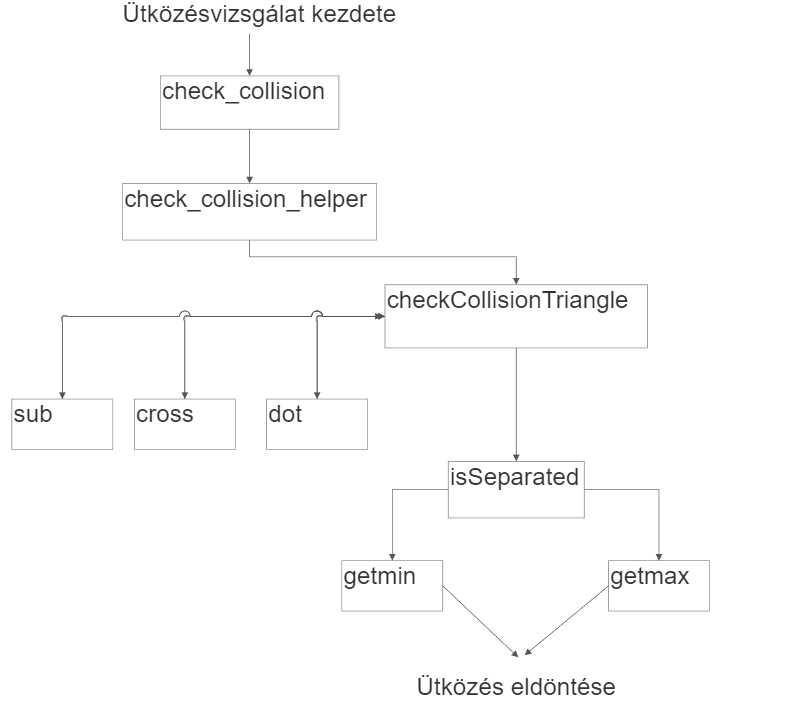
\includegraphics[width=15truecm, height=15truecm]{images/blokk_diagram.png}
	\caption{Függvénykönyvtár hívási fája}
	\label{fig:blokkdiagram}
\end{figure}




\newpage


\Section{Demo program működtetése}
\label{chap:demo}
A függvénykönyvtár teszteléséhez készítettem egy programot, amellyel szemléltethetjük a számításokat, a számítások működését és azok hatékonyságát. A teszt programban egy úgynevezett "playermodel"\textsuperscript{\ref{def:playermodel}}-t irányíthatunk, amely egy egyszerű kocka modell. A playermodellel\textsuperscript{\ref{def:playermodel}} körbejárhatjuk a teret, a modellt forgathatjuk, tükrözhetjük, méretezhetjük, illetve más modellekkel ütközhetünk. A program működtetéséhez használható különböző billentyűkombinációkat a \ref{tab:demo} táblázat szemlélteti.

\begin{table}[h]
	\centering
	\begin{tabular}{|l|l|}
		\hline
		\multicolumn{1}{|c|}{\textbf{Billentyű}} & \multicolumn{1}{c|}{\textbf{Esemény}}\\
		\hline
		W,A,S,D & {A "playermodel"\textsuperscript{\ref{def:playermodel}} mozgatása a térben X,Y tengelyen.} \\\hline
		CTRL, SPACE & A "playermodel"\textsuperscript{\ref{def:playermodel}} mozgatása a térben Z tengelyen. \\\hline
		Egér & A kamera mozgatása a "playermodel"\textsuperscript{\ref{def:playermodel}} körül. \\\hline
		Görgő & A kamera távolságának állítása a "playermodelhez"\textsuperscript{\ref{def:playermodel}} képest. \\\hline
		E & Új modell létrehozása az ütközésvizsgálat teszteléséhez. \\\hline
		Q & A "playermodel"\textsuperscript{\ref{def:playermodel}}, illetve a "hitbox"\textsuperscript{\ref{def:hitbox}} ki/be kapcsolása. \\\hline
		ESC & Kilépés a programból. \\\hline
		N, M & A "playermodel"\textsuperscript{\ref{def:playermodel}} méretének növelése/csökkentése. \\\hline
		C, V, B & A "playermodel"\textsuperscript{\ref{def:playermodel}} tükrözése X, Y és Z tengelyekre. \\\hline
		J, L & A "playermodel"\textsuperscript{\ref{def:playermodel}} forgatása az X tengelyen. \\\hline
		I, K & A "playermodel"\textsuperscript{\ref{def:playermodel}} forgatása az Y tengelyen. \\\hline
		U, O & A "playermodel"\textsuperscript{\ref{def:playermodel}} forgatása az Z tengelyen. \\\hline
	\end{tabular}
	\caption{Demo program használata}
	\label{tab:demo}
\end{table}

\newpage
\Chapter{Optimalizálás}

Minél több a "playermodel"\textsuperscript{\ref{def:playermodel}} háromszögeinek száma, illetve a többi modellek száma, és azok háromszögeinek száma, annál több számítást kell végeznünk. Például 2 modell esetén, ha a playermodellünk\textsuperscript{\ref{def:playermodel}} 100 háromszögből áll, és a másik modellünk is szintén 100 háromszögből áll, akkor a programnak frame-enként 100$\cdot$100, azaz $10\,000$ számítást kell végeznie, négyzetes idejű az algoritmus számítási ideje. Emiatt a módszer nem alkalmas valós idejű alkalmazásokhoz. Több módszert is kipróbáltam lehetséges optimalizálás szempontjából.

\Section{Szűrés távolság alapján}
Minden modell betöltésekkor kiszámítjuk a modell középpontjától számított legtávolabbi pontjának hosszát, ahogy a \ref{fig:opt_1} ábrán láthatjuk. Ezt csak egyszer kell kiszámítanunk, kivéve ha futtatás közben szeretnénk módosítani a modellt, például a modell méretének megváltoztatásával. Ütközésvizsgálat előtt kiszámítjuk, hogy a két modell ütközhet-e egymással vagy sem. Ez lényegében a négyzetes elválasztás(\ref{chap:quad}) módszere alapján működik.
\\
Részlet a check\_collision függvényből:
\begin{cpp}
float limit, distance;
limit = model1->farestpoint + model2->farestpoint + 0.5;
distance = get_distance(model1_position, model2_position);
if (fminf(distance, limit) == limit)
{
    return false;
}
\end{cpp}

\vfill
\begin{definition}[Playermodel]
	A "playermodel" egy számítógépes játékban használt grafikus megjelenítése a játékos karakternek, amely magában foglalja annak kinézetét és animációit a játék világában való mozgása során.
	\label{def:playermodel}
\end{definition}
\newpage
A limit változóban megnézzük a maximális távolságot, amelyen belül már ütközésvizsgálatot vizsgálunk. Összeadjuk a két modell legtávolabbi pontjának távolságát, illetve egy extra konstanst. Ezután a distance változóba elmentjük a két modell közötti távolságot. Ha a limit kisebb, mint a distance, akkor nem lehetséges a két modell ütközése, azért visszatérünk false értékkel, nem vizsgálunk ütközést.

Az optimalizálás ezen esetben \textbf{sikeres}, kevesebb számítást veszünk figyelembe, a program gyorsul, amely függ a modellek távolságától, méretétől és komplexitásától.
\begin{figure}[h]
	\centering
	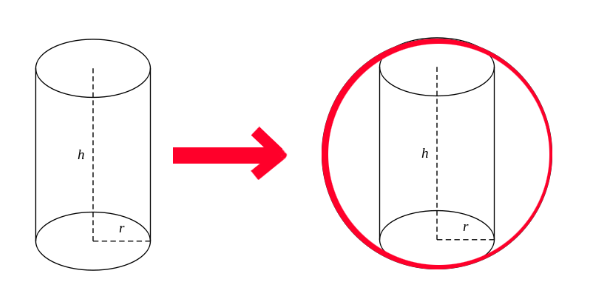
\includegraphics[width=13truecm, height=7.5truecm]{images/opt_5.1.png}
	\caption{Modell köré egy gömb alakú "hitbox"\textsuperscript{\ref{def:hitbox}} generálása}
	\label{fig:opt_1}
\end{figure}

\newpage
\Section{Távolság szűrése háromszögekkel}
\label{opt_tav}
Lényege, hogy ütközésvizsgálat előtt a modellek háromszögeinek a középpontját kiszámítjuk, majd a középpontokat viszonyítjuk egymáshoz, ahogy a \ref{fig:opt_2} ábrán láthatjuk. Ha a háromszögek közötti távolság nagyobb, mint a maximum táv, akkor az adott háromszög számítása elhanyagolható, mivel biztosra vehetjük, hogy nem lesz az adott két háromszög esetén metszés.

Az optimalizálás ezen esetben sikertelen, a számítások ideje drasztikusan megnő, használata nem ajánlott.

\Section{Távolság szűrése háromszögek mentésével}
Lényege ugyan az, mint az előző szekcióban bemutatott algoritmusnak, annyi kivétellel, hogy a középpontokat csak a modell beolvasásakor számítjuk ki, majd lementjük későbbi használatra, ahogy a \ref{fig:opt_2} ábrán láthatjuk.

Az optimalizálás ezen esetben sikertelen, a számítások ideje megnő az optimalizálatlan programhoz képest, de csökken az \ref{opt_tav} algoritmushoz képest, illetve 25\%-al megnő a memóriaigény is. Használata nem ajánlott.
\begin{figure}[h]
	\centering
	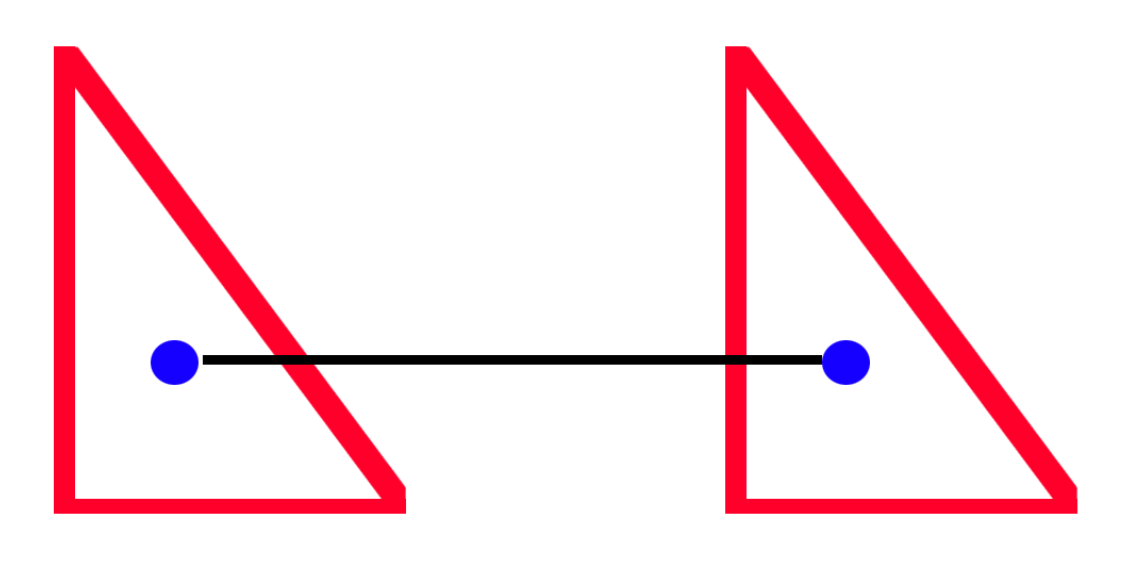
\includegraphics[width=13truecm, height=7.5truecm]{images/opt_5.2.png}
	\caption{Távolság szűrése háromszögek középpontjával}
	\label{fig:opt_2}
\end{figure}

\newpage
\Section{Pozíció alapján szűrés}
Lényege, hogy az adott modell nem feltétlenül van mindig ugyan abban a síkban, mint a másik vizsgálandó modell. Megnézzük a két modell középpontjának koordinátáit, illetve a legtávolabbi pontját az adott tengelyhez képest, ahogy az \ref{fig:opt_3} ábrán láthatjuk. Például, ha a playermodellünk a Z koordinátán 20 pixel magas, akkor a maximum szint a Z tengelyen az a modell középpontja + 20 pixel lesz, minden más háromszöget az adott modellben figyelmen kívül hagyunk. Ezeket a lépéseket meg kell ismételnünk minden tengelyre 2 alkalommal. Ez összesen 6 különböző számítást jelent.

Az optimalizálás ezen esetben megoldható, a számítások ideje csökken, de cserébe a memória igény nő.
\begin{figure}[h]
	\centering
	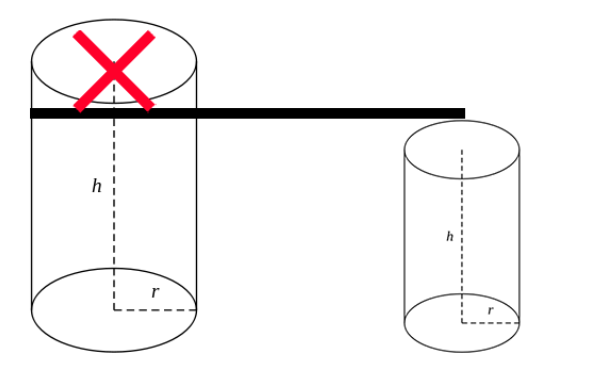
\includegraphics[width=13truecm, height=7.5truecm]{images/opt_5.3.png}
	\caption{Tengelyek alapján szűrés}
	\label{fig:opt_3}
\end{figure}

\Chapter{Demo program működtetése}

A függvénykönyvtár teszteléséhez készült egy program, amellyel szemléltethetjük a számításokat, a számítások működését és azok hatékonyságát. A teszt programban egy úgynevezett "playermodell"-t irányíthatunk, amely egy egyszerű kocka modell. A playermodellel körbejárhatjuk a teret, a modellt forgathatjuk, tükrözhetjük, méretezhetjük, illetve más modellekkel ütközhetünk. Ezen lépésekhez különböző billentyűkombinációk érhetőek el.
\begin{table}[h]
	\centering
	\begin{tabular}{|l|l|}
		\hline
		\multicolumn{1}{|c|}{\textbf{Billentyű}} & \multicolumn{1}{c|}{\textbf{Esemény}}\\
		\hline
		 W,A,S,D & {A "playermodell" mozgatása a térben X,Y tengelyen.} \\\hline
		 CTRL, SPACE & A "playermodell" mozgatása a térben Z tengelyen. \\\hline
		 Egér & A kamera mozgatása a "playermodell" körül. \\\hline
		 Görgő & A kamera távolságának állítása a "playermodellhez" képest. \\\hline
		 E & Új modell létrehozása az ütközésvizsgálat teszteléséhez. \\\hline
		 Q & A "playermodell", illetve a "hitbox" ki/be kapcsolása. \\\hline
		 ESC & Kilépés a programból. \\\hline
		 N, M & A "playermodell" méretének növelése/csökkentése. \\\hline
		 C, V, B & A "playermodell" tükrözése X, Y és Z tengelyekre. \\\hline
		 J, L & A "playermodell" forgatása az X tengelyen. \\\hline
		 I, K & A "playermodell" forgatása az Y tengelyen. \\\hline
		 U, O & A "playermodell" forgatása az Z tengelyen. \\\hline
	\end{tabular}
\end{table}

\newpage
\Chapter{Összefoglalás}

A szakdolgozat eredménye egy könnyen használható függvénykönyvtár, amely lehetővé teszi 3 dimenziós modellek beimportálását, valamint "hitbox"\textsuperscript{\ref{def:hitbox}}-ként kezelését, ütközések vizsgálatát más modellekkel. A program fejlesztése során kiemelt figyelmet kapott, hogy az alkalmazást könnyen használhassák más fejlesztők, akik esetleg nem jártasak, vagy csak kevés tapasztalattal rendelkeznek ütközések vizsgálatában.

A beépített funkciók azonnal elérhetővé válnak, amint beimportáljuk a függvénykönyvtárat a fejlesztői környezetbe. Fontos megemlítenünk, hogy a függvénykönyvtár használatához a fejlesztőnek szüksége van egy C fordítóra, illetve rendelkeznie kell OpenGL \cite{OpenGL} és SDL2 \cite{SDL2} függvénykönyvtárakkal is. A fejlesztő döntheti el, hogy mikor és milyen modellekre alkalmazza a vizsgálatot, illetve milyen eseményekkel jár az ütközés, ezzel személyre szabható a program minden része.

Az ütközésvizsgálat egyszerűen elvégezhető a check\_collision függvény meghívásával, illetve a szükséges adatok megadásával. A függvény eredményeként visszatér egy igaz, vagy hamis értékkel, ezzel jelezve, hogy a modellek ütköztek-e egymással, vagy sem.

A jövőben számos további fejlesztés valósulhat meg a program szempontjából, ilyen lehet például az optimalizálás, amellyel a teljesítményt növelhetjük, míg az erőforrások nagyságát csökkenthetjük, valamint még könnyebbé, felhasználóbarátabbá tehetjük a program használatát.

A függvénykönyvtár széles körben alkalmazható fizikai szimulációk, videójátékok esetében, ezzel hozzájárulva a fejlesztők munkájához, illetve a számítógépes grafikában rejlő lehetőségek kiaknázásához.

\clearpage

\addcontentsline{toc}{chapter}{Irodalomjegyzék}
\bibliographystyle{plain}
\bibliography{dolgozat.bib}

\newpage

\pagestyle{empty}

\noindent \textbf{\Large CD Használati útmutató}

\vskip 1cm

A függvénykönyvtár használatához szükségünk van egy OpenGL alapú programra. Amennyiben nem rendelkezünk ilyennel, a szakdolgozat tartalmaz egy demo programot, amelyen tesztelhetjük a funkciókat.

A demo elindításához nem kell mást tennünk, mint elindítani a start.bat file-t a program nevezetű mappában.

A CD lemez tartalmazza:
\begin{itemize}
\item a dolgozatot egy \texttt{dolgozat.pdf} fájl formájában,
\item a LaTeX forráskódját a dolgozatnak a szakdolgozat nevezetű mappában,
\item az elkészített programot a program nevezetű mappában,
\item a használt matematikai képletet tartalmazó pdf-et DynamicCollisionDetection néven,
\item egy útmutatót a CD használatához README.md néven.
\end{itemize}


\end{document}
